\chapter{Επίπεδα Signal2Image σε βαθιά νευρωνικά δίκτυα για ταξινόμηση EEG}
\label{chapter5}
\graphicspath{{./images/signal2image-modules-in-deep-neural-networkds-for-eeg-classification/}}

\section{Εισαγωγή}
Η βαθιά μάθηση έχει φέρει επανάσταση στην όραση υπολογιστών, χρησιμοποιώντας την αυξημένη διαθεσιμότητα βάσεων δεδομένων μεγάλου όγκου και τη δύναμη των παράλληλων υπολογιστικών μονάδων, όπως είναι οι μονάδες επεξεργασίας γραφικών.
Η συντριπτική πλειοψηφία της έρευνας στην βαθιά μάθηση γίνεται με τη χρήση εικόνων ως δεδομένων εκπαίδευσης, ωστόσο ο βιοϊατρικός τομέας είναι πλούσιος σε σήματα φυσιολογίας που χρησιμοποιούνται για προβλήματα διάγνωσης και πρόβλεψης.
Είναι ακόμα ανοιχτό ερευνητικό ερώτημα, η καλύτερη αξιοποίηση σημάτων για την εκπαίδευση βαθιών νευρωνικών δικτύων.

Οι περισσότερες μέθοδοι για την επίλυση βιοϊατρικών προβλημάτων μέχρι πρόσφατα, περιελάμβαναν χειροποίητη δημιουργία χαρακτηριστικών και προσπάθεια μίμησης ανθρώπινων εμπειρογνωμόνων, τα οποία αποδεικνύονται όλο και περισσότερο ανεπαρκή και επιρρεπή σε σφάλματα.
Η βαθιά μάθηση αναδεικνύεται ως μια ισχυρή λύση για ένα ευρύ φάσμα προβλημάτων στη βιοϊατρική, που επιτυγχάνει καλύτερα αποτελέσματα σε σύγκριση με την παραδοσιακή μηχανική μάθηση.
Το κύριο πλεονέκτημα των μεθόδων που χρησιμοποιούν τη βαθιά μάθηση είναι ότι μαθαίνουν ιεραρχικά χαρακτηριστικά από δεδομένα εκπαίδευσης με αυτόματο τρόπο, κάτι το οποίο τα καθιστά πιο κλιμακωτά και γενικεύσιμα από παραδοσιακές μεθόδους.
Αυτό επιτυγχάνεται με τη χρήση δικτύων πολλαπλών επιπέδων που αποτελούνται από εκατομμύρια παραμέτρους~\cite{krizhevsky2012imagenet}, εκπαιδευμένα με backpropagation~\cite{rumelhart1986learning} σε μεγάλο όγκο δεδομένων.
Παρόλο που η βαθιά μάθηση χρησιμοποιείται κυρίως σε βιοϊατρικές εικόνες υπάρχει επίσης ένα ευρύ φάσμα φυσιολογικών σημάτων, όπως το EEG, τα οποία χρησιμοποιούνται για προβλήματα διάγνωσης και πρόβλεψης.
Το EEG είναι μια μέτρηση του ηλεκτρικού πεδίου που παράγεται από τον εγκέφαλο και χρησιμοποιείται για την ταξινόμηση σταδίων του ύπνου~\cite{aboalayon2016sleep}, τις διεπαφές υπολογιστή-εγκεφάλου~\cite{al2017review}, την συναισθηματική παρακολούθηση~\cite{lotte1999electroencephalography} και την ταξινόμηση της επιληψίας~\cite{acharya2013automated}.

Οι Yannick et al.~\cite{yannick2019deep} εξέτασαν δημοσιεύσεις βαθιάς μάθησης με χρήση του EEG και εντόπισαν μια γενική αύξηση της ακρίβειας όταν χρησιμοποιείται βαθιά μάθηση και συγκεκριμένα όταν χρησιμοποιούνται CNN αντί παραδοσιακών μεθόδων μηχανικής μάθησης.
Ωστόσο δεν αναφέρουν συγκεκριμένα χαρακτηριστικά των αρχιτεκτονικών CNN που ευθύνονται για την αύξηση της απόδοσης.
Είναι ακόμα ανοιχτό ερευνητικό ερώτημα, το πως μπορεί να χρησιμοποιηθεί το EEG για την εκπαίδευση μοντέλων βαθιάς μάθησης.

Μια κοινή προσέγγιση που χρησιμοποίησαν προηγούμενες μελέτες για την ταξινόμηση των σημάτων EEG ήταν η εξαγωγή χαρακτηριστικών από το πεδίο συχνοτήτων και χρόνου--συχνοτήτων, που χρησιμοποιούν τη θεωρία πίσω από τις συχνότητες των ζωνών EEG~\cite{langkvist2012sleep}: δέλτα (0.5--4 Hz), θήτα (4--8 Hz), άλφα (8--13 Hz), βήτα (13--20 Hz) και γάμμα (20--64 Hz).
Οι Truong et al.~\cite{truong2018convolutional} χρησιμοποίησαν STFT σε παράθυρο ολίσθησης 30 δευτερολέπτων, για να εκπαιδεύσουν ένα CNN τριών επιπέδων σε αναπαραστάσεις πεδίου χρόνου-συχνοτήτων, για πρόβλεψη επιληπτικών κρίσεων και αξιολόγησαν τη μέθοδο τους σε τρεις βάσεις δεδομένων EEG\@.
Οι Khan et al.~\cite{khan2018focal} μετασχημάτισαν τα EEG στο πεδίο χρόνου-συχνοτήτων χρησιμοποιώντας κυματίδια πολλαπλών κλιμάκων και έπειτα εκπαίδευσαν ένα CNN έξι επιπέδων, για την πρόβλεψη της εστιακής έναρξης παρουσιάζοντας υποσχόμενα αποτελέσματα.

Η εξαγωγή χαρακτηριστικών από το πεδίο χρόνου-συχνοτήτων έχει επίσης χρησιμοποιηθεί και σε άλλες δημοσιεύσεις που σχετίζονται με το EEG, εκτός από την πρόγνωση επιληπτικών κρίσεων.
Οι Zhang et al.~\cite{zhang2017pattern} εκπαίδευσαν ένα ensemble CNN που περιείχε δύο έως δέκα επίπεδα, χρησιμοποιώντας χαρακτηριστικά STFT που εξήχθησαν από τις EEG συχνότητες για ταξινόμηση ψυχικού φόρτου εργασίας.
Οι Giri et al.~\cite{giri2016ischemic} εξήγαγαν στατιστικά και μέτρα πληροφορίας από το πεδίο συχνοτήτων για την εκπαίδευση ενός 1D CNN με δύο επίπεδα, για τον εντοπισμό ισχαιμικού εγκεφαλικού επεισοδίου.

Σε αυτό το κεφάλαιο και στο πλαίσιο της διδακτορικής διατριβής ορίζουμε τα επίπεδα νευρωνικών δικτύων Signal2Image (S2I) ως κάθε δομικό στοιχείο που τοποθετείται μετά την είσοδο μη-επεξεργασμένου σήματος και πριν από ένα `μοντέλο βάσης' που είναι συνήθως μια καθιερωμένη αρχιτεκτονική για προβλήματα εικόνων.
Μία σημαντική ιδιότητα ενός S2I είναι αν αποτελείται από παραμέτρους που μπορούν να εκπαιδευτούν όπως συνελικτικά και γραμμικά επίπεδα ή είναι μη-εκπαιδεύσιμα όπως οι παραδοσιακές μέθοδοι χρόνου-συχνοτήτων.
Χρησιμοποιώντας αυτόν τον ορισμό μπορούμε επίσης να καταλήξουμε στο συμπέρασμα ότι οι περισσότερες προηγούμενες μέθοδοι για την ταξινόμηση EEG χρησιμοποιούν μη-εκπαιδεύσιμα S2I και ότι καμία προηγούμενη μελέτη δεν έχει συγκρίνει εκπαίδευσιμα με μη-εκπαιδεύσιμα S2I.

Συγκρίνουμε τα εκπαιδεύσιμα και μη-εκπαιδεύσιμα S2Is σε συνδυασμό με τις γνωστές αρχιτεκτονικές νευρωνικών δικτύων `μοντέλων βάσης', μαζί με τις 1D και τις σε βάθος παραλλαγές των τελευταίων.
Μια επισκόπηση υψηλού επιπέδου αυτών των συνδυασμένων μεθόδων παρουσιάζεται στην Εικ.~\ref{fig:highleveloverview}.
Αν και επιλέγουμε το σύνολο δεδομένων αναγνώρισης επιληπτικών ελλείψεων EEG από το Πανεπιστήμιο της Καλιφόρνιας, Irvine (University of California, UCI)~\cite{andrzejak2001indications} για ταξινόμηση EEG, οι συνέπειες αυτής της μελέτης θα μπορούσαν να γενικευτούν σε οποιοδήποτε είδος προβλήματος ταξινόμησης σημάτων.
Εδώ επίσης αναφερόμαστε στο CNN ως ένα νευρωνικό δίκτυο που αποτελείται από εναλλασσόμενα συνελικτικά επίπεδα ακολουθούμενα από ένα ReLU και ένα επίπεδο μέγιστης συγκέντρωσης και ένα πλήρως συνδεδεμένο επίπεδο στο τέλος, ενώ ο όρος `επίπεδο' υποδηλώνει τον αριθμό των συνελικτικών επιπέδων.

\section{Δεδομένα}
Η βάση δεδομένων αναγνώρισης επιληπτικών κρίσεων UCI EEG~\cite{andrzejak2001indications} αποτελείται από $500$ σήματα το καθένα με $4097$ δείγματα (23.5 δευτερόλεπτα).
Αποτελείται από πέντε κατηγορίες με $100$ σήματα για κάθε κλάση (σε παρένθεση τα συντομευμένα ονόματα των επισημάνσεων που χρησιμοποιούνται στα Σχήματα~\ref{fig:highleveloverview} και~\ref{fig:signal2imageoutputs}):
\begin{enumerate}
	\item υγιής ασθενής ενώ έχει τα μάτια του ανοιχτά (Open),
	\item υγιής ασθενής, έχοντας τα μάτια κλειστά (Closed),
	\item ασθενής με όγκο με σήμα που λαμβάνεται από υγιή περιοχή (Healthy),
	\item ασθενής με όγκο με σήμα που λαμβάνεται από την περιοχή του όγκου (Tumor),
	\item ασθενής ενώ έχει επιληπτική δραστηριότητα (Epilepsy)
\end{enumerate}

Για τους σκοπούς αυτού του κεφαλαίου χρησιμοποιούμε μια παραλλαγή της βάσης δεδομένων\footnote{\url{https://archive.ics.uci.edu/ml/datasets/Epileptic+Seizure+Recognition}} στην οποία τα σήματα EEG χωρίζονται σε τμήματα με $178$ δείγματα το καθένα, καταλήγοντας σε ένα ισορροπημένο σύνολο δεδομένων που αποτελείται από $11500$ σήματα EEG\@.

\begin{figure}
	\centering
	\begin{tikzpicture}[]
		\node[] at (-4.5, 0){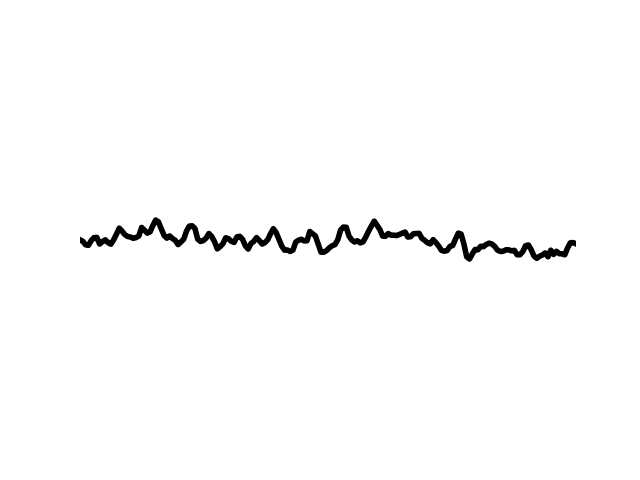
\includegraphics[scale=0.2,angle=90]{signal_epilepsy.png}};
		\node[align=left] at (-4.2, 0) {$x_i$};
		\draw[dashed,->] (-4, 0) -- (-3.8, 0);
		\node[draw, minimum height=2.55cm] at (-3.5, 0) {$m$};
		\draw[dashed,->] (-3.2, 0) -- (-3, 0);
		\node[] at (-1.7, 0){
\includegraphics[scale=0.41,angle=90]{cnn_epilepsy.png}};
		\draw[dashed,->] (-0.4, 0) -- (-0.2, 0);
		\node[draw, minimum height=2.55cm] at (0.1, 0) {$b_d$};
		\draw[dashed,->] (0.4, 0) -- (0.6, 0);
		\node[align=left] at (0.8, 0) {$\hat{y_i}$};
		\node[minimum width=0.5cm, minimum height=0.5cm] at (2, 1.1) {\footnotesize Open 0.1\%};
		\node[minimum width=0.5cm, minimum height=0.5cm] at (2, 0.55) {\footnotesize Closed 0.2\%};
		\node[minimum width=0.5cm, minimum height=0.5cm] at (2, 0) {\footnotesize Healthy 0.9\%};
		\node[minimum width=0.5cm, minimum height=0.5cm] at (2, -0.55) {\footnotesize Tumor 34.7\%};
		\node[minimum width=0.5cm, minimum height=0.5cm] at (2, -1.1) {\footnotesize Epilepsy 64.1\%};
	\end{tikzpicture}
	\caption[Αρχιτεκτονική Signal2Image]{Αρχιτεκτονική Signal2Image.
	$x_i$ είναι η είσοδος, $m$ είναι το Signal2Image, $b_d$ είναι η 1D ή 2D αρχιτεκτονική του `μοντέλου βάσης' για $d=1,2$ αντίστοιχα και $\hat{y_i}$ είναι η προβλεπόμενη έξοδος.
	Τα ονόματα των επισημάνσεων απεικονίζονται δεξιά μαζί με τις προβλέψεις για το απεικονιζόμενο σήμα.
	Η εικόνα μεταξύ του $m$ και του $b_d$ απεικονίζει την έξοδο του CNN Signal2Image ενός επιπέδου, ενώ το `σήμα ως εικόνα' και φασματογράφημα έχουν ενδιάμεσες εικόνες όπως απεικονίζονται στην δεύτερη και τρίτη σειρά του σχήματος~\ref{fig:signal2imageoutputs}.
	Τα βέλη απεικονίζουν την ροή της προς-τα-εμπρός διάδοσης.
	Για την 1D αρχιτεκτονική το $m$ παραλείπεται και δεν δημιουργείται ενδιάμεση εικόνα.}
	\label{fig:highleveloverview}
\end{figure}

\section{Μέθοδοι}
\subsection{Ορισμοί}
Ορίζουμε το σύνολο δεδομένων $D=\{x_i, y_i\}_{i=1\ldots N}$ όπου $x_i \in \mathbb{Z}^n$ και $y_i \in \{1, 2, 3, 4, 5\}$ υποδηλώνει το $i^{th}$ σήμα εισόδου με διαστάσεις $n=178$ και την $i^{th}$ επισήμανση με πέντε πιθανές κατηγορίες αντίστοιχα.
$N=11500$ είναι ο αριθμός των παρατηρήσεων.

Επίσης, ορίζουμε το σύνολο των S2Is ως $M$ και το μέλος αυτού του συνόλου ως $m$ το οποίο περιλαμβάνει τα ακόλουθα:
\begin{itemize}
	\item 'σήμα ως εικόνα' (μη-εκπαιδεύσιμο)
	\item φασματογράφημα (μη-εκπαιδεύσιμο)
	\item CNN ενός και δύο επιπέδων (εκπαιδεύσιμο)
\end{itemize}

Καθορίζουμε στη συνέχεια το σύνολο των `μοντέλων βάσης' ως $B$ και το μέλος αυτού του συνόλου ως $b_d$ όπου $d=[1,2]$ υποδηλώνει τη διαστασιμότητα των επιπέδων συνέλιξης (convolutional), μέγιστης συγκέντρωσης (max-pooling) και κανονικοποίησης παρτίδας (batch-norm).
Το $B$ περιλαμβάνει τα παρακάτω $b_d$ μαζί με τις παραλλαγές σε βάθος και τις ισοδύναμες 1D αρχιτεκτονικές για $d=1$ (για μια πλήρη λίστα ανατρέξτε στις δύο πρώτες σειρές του Πίνακα.~\ref{table:results}):
\begin{itemize}
	\item LeNet~\cite{lecun1998gradient}
	\item AlexNet~\cite{krizhevsky2012imagenet}
	\item VGGnet~\cite{simonyan2014very}
	\item ResNet~\cite{he2016deep}
	\item DenseNet~\cite{huang2017densely}
\end{itemize}

Τέλος ορίσαμε τους συνδυασμούς των $m$ και $b_d$ ως μέλη $c$ του συνόλου συνδυασμένων μοντέλων $C$.
Χρησιμοποιώντας τους προηγούμενους ορισμούς, ο στόχος αυτού του κεφαλαίου είναι η αξιολόγηση του συνόλου των μοντέλων $C$, όπου $C$ είναι το συνδυασμένο σύνολο των $M$ και $B$ δλδ. $C=M\times B$ σε σχέση με την χρονική απόδοση και την ακρίβεια εκπαιδευμένα στο $D$.

\subsection{Signal2Image}
Σε αυτή την ενότητα περιγράφονται τα εσωτερικά στοιχεία κάθε μονάδας S2I.
Για το S2I `σήμα ως εικόνα' κανονικοποιήσαμε το πλάτος $x_i$ στο εύρος $[1, 178]$.
Τα αποτελέσματα αντιστράφηκαν κατά μήκος του άξονα y, στρογγυλοποιημένα στον πλησιέστερο ακέραιο και στη συνέχεια χρησιμοποιήθηκαν ως y-δείκτες για τα εικονοστοιχεία με πλάτος $255$ σε μια εικόνα $178\times 178$ αρχικοποιημένη με μηδενικά.

Για το S2I φασματογράφου, το οποίο χρησιμοποιείται για την απεικόνιση της μεταβολής της συχνότητας ενός μη-στάσιμου σήματος με την πάροδο του χρόνου~\cite{oppenheim1999discrete}, χρησιμοποιήθηκε παράθυρο Tukey με παράμετρο σχήματος $0.25$, μήκος τμήματος $8$ δειγμάτων, αλληλεπικάλυψη μεταξύ τμημάτων $4$ δειγμάτων και ταχύ Μετασχηματισμό Fourier των $64$ δειγμάτων για την μετατροπή του $x_i$ στο πεδίο χρόνου-συχνοτήτων.
Το προκύπτων φασματογράφημα, το οποίο αντιπροσωπεύει το μέγεθος της φασματικής πυκνότητας ισχύος ($V^2/Hz$) του $x_i$, στη συνέχεια υπερδειγματολήφθηκε σε $178\times 178$ με χρήση διγραμμικής παρεμβολής μεταξύ των εικονοστοιχείων.

Για τα S2I CNN με ένα και δύο επίπεδα, το $x_i$ μετατρέπεται σε εικόνα χρησιμοποιώντας εκπαιδεύσιμες παραμέτρους, αντί χρήσης κάποιας στατικής διαδικασίας.
Το S2I ενός επιπέδου αποτελείται από ένα 1D συνελικτικό επίπεδο (μεγέθη πυρήνα $3$ με $8$ κανάλια).
Το S2I δύο επιπέδων αποτελείται από δύο 1D συνελικτικά επίπεδα (μεγέθη πυρήνα $3$ με $8$ και $16$ κανάλια) με το πρώτο επίπεδο να ακολουθείται από μια συνάρτηση ενεργοποίησης ReLU και ένα επίπεδο 1D max-pooling (μέγεθος πυρήνα $2$).
Οι χάρτες ενεργοποιήσεων του τελευταίου συνελικτικού επιπέδου και για τα δύο S2I συμπτύσσονται σειριακά κατά μήκος του y-άξονα και στη συνέχεια μετατρέπονται σε μέγεθος $178\times 178$ χρησιμοποιώντας τη διγραμμική παρεμβολή.

Περιορίζουμε την έξοδο για όλα τα $m$ σε μια εικόνα μεγέθους $178\times 178$ για να επιτρέψουμε οπτική σύγκριση.
Τρία πανομοιότυπα κανάλια στοιβάζονται επίσης για όλες τις εξόδους των $m$ για να ικανοποιήσουν τις απαιτήσεις μεγέθους εισόδου των $b_d$.
Οι αρχιτεκτονικές όλων των $b_d$ παραμένουν οι ίδιες, εκτός του αριθμού των εξόδων του τελευταίου γραμμικού επιπέδου που έχει οριστεί σε πέντε για να αντιστοιχεί στον αριθμό των κατηγοριών του $D$.
Ένα παράδειγμα των αντίστοιχων εξόδων κάποιων από τα $m$ (το CNN ενός/δύο επιπέδων παρήγαγαν παρόμοιες απεικονίσεις) απεικονίζονται στη δεύτερη, τρίτη και τέταρτη σειρά του σχήματος~\ref{fig:signal2imageoutputs}.

\begin{figure}
	\centering
	\subfloat{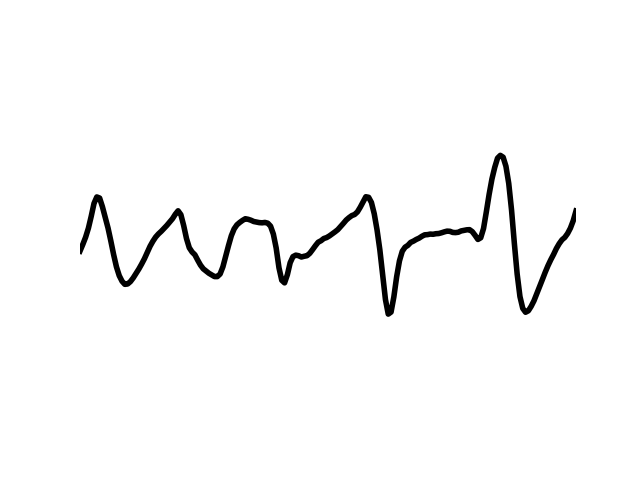
\includegraphics[scale=0.16]{signal_eyes_open.png}}
	\quad
	\subfloat{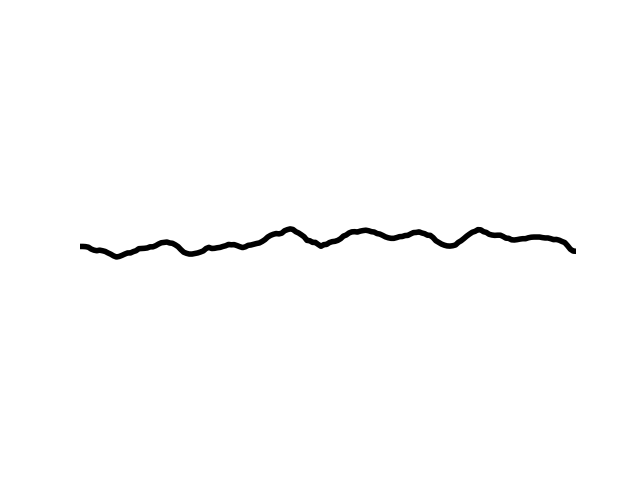
\includegraphics[scale=0.16]{signal_eyes_closed.png}}
	\quad
	\subfloat{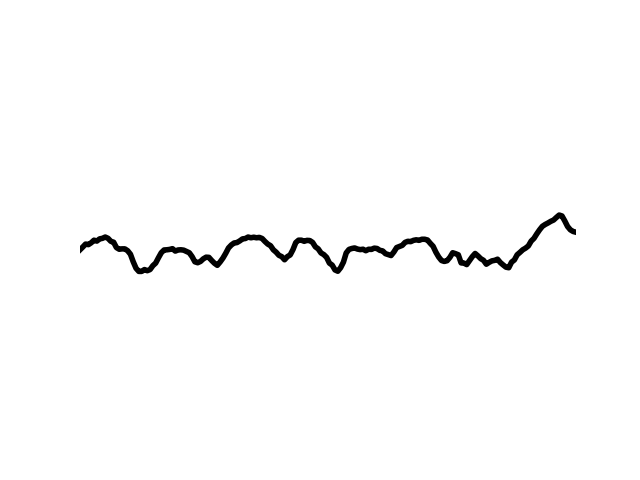
\includegraphics[scale=0.16]{signal_healthy_area.png}}
	\quad
	\subfloat{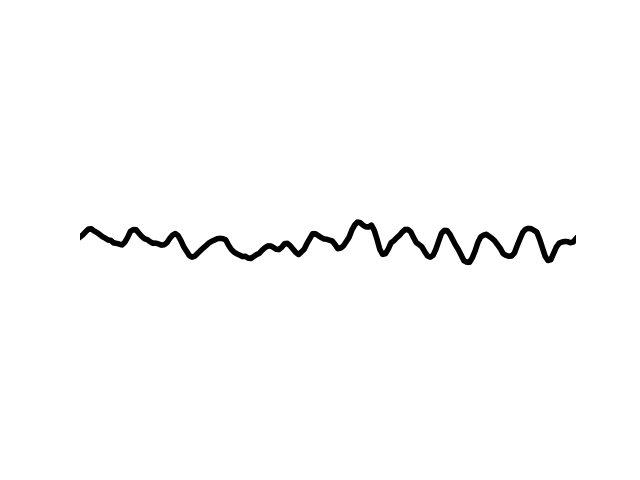
\includegraphics[scale=0.16]{signal_tumor_area.png}}
	\quad
	\subfloat{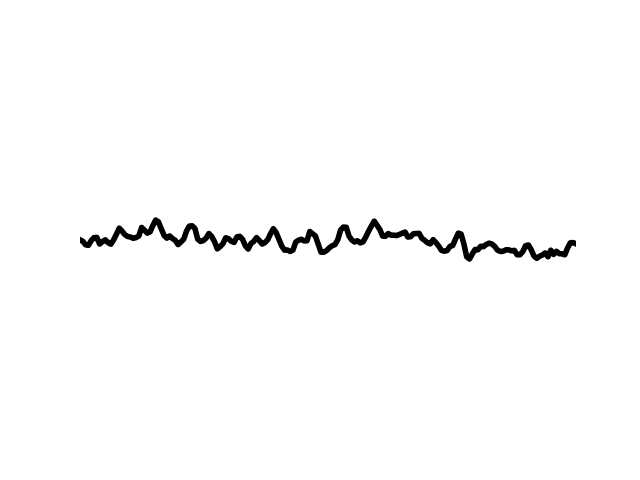
\includegraphics[scale=0.16]{signal_epilepsy.png}}
	\\
	\subfloat{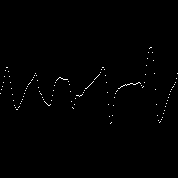
\includegraphics[scale=0.42]{signal_as_image_eyes_open.png}}
	\quad
	\subfloat{
\includegraphics[scale=0.42]{signal_as_image_eyes_closed.png}}
	\quad
	\subfloat{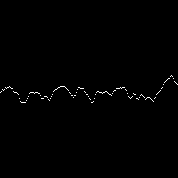
\includegraphics[scale=0.42]{signal_as_image_healthy_area.png}}
	\quad
	\subfloat{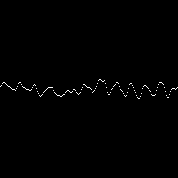
\includegraphics[scale=0.42]{signal_as_image_tumor_area.png}}
	\quad
	\subfloat{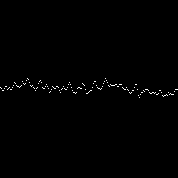
\includegraphics[scale=0.42]{signal_as_image_epilepsy.png}}
	\\
	\subfloat{
\includegraphics[scale=0.42]{spectrogram_eyes_open.png}}
	\quad
	\subfloat{
\includegraphics[scale=0.42]{spectrogram_eyes_closed.png}}
	\quad
	\subfloat{
\includegraphics[scale=0.42]{spectrogram_healthy_area.png}}
	\quad
	\subfloat{
\includegraphics[scale=0.42]{spectrogram_tumor_area.png}}
	\quad
	\subfloat{
\includegraphics[scale=0.42]{spectrogram_epilepsy.png}}
	\\
	\setcounter{subfigure}{0}
	\subfloat[Open]{
\includegraphics[scale=0.42]{cnn_eyes_open.png}}
	\quad
	\subfloat[Closed]{
\includegraphics[scale=0.42]{cnn_eyes_closed.png}}
	\quad
	\subfloat[Healthy]{
\includegraphics[scale=0.42]{cnn_healthy_area.png}}
	\quad
	\subfloat[Tumor]{
\includegraphics[scale=0.42]{cnn_tumor_area.png}}
	\quad
	\subfloat[Epilepsy]{
\includegraphics[scale=0.42]{cnn_epilepsy.png}}
	\caption[Σήματα και έξοδοι των Signal2Image για κάθε κλάση]{Σήματα και έξοδοι των Signal2Image για κάθε κλάση.
	Οι x, y-άξονες της πρώτης σειράς είναι \SI{}{\micro V} και χρονικά δείγματα αντίστοιχα.
	Οι x, y-άξονες των υπόλοιπων εικόνων απεικονίζουν χωρική πληροφορία, επειδή δεν ενημερώνουμε το `μοντέλο βάσης' με την έννοια του χρόνου κατά τον x-άξονα ή την έννοια της συχνότητας κατά τον y-άξονα.
	Υψηλότερη ένταση των εικονοστοιχείων υποδηλώνει υψηλότερο πλάτος.}
	\label{fig:signal2imageoutputs}
\end{figure}

\section{Ρύθμιση πειραμάτων}
Τα συνελικτικά επίπεδα αρχικοποιήθηκαν με χρήση ομοιόμορφου θορύβου τύπου Kaiming~\cite{he2015delving}. Οι τιμές λαμβάνονται από την ομοιόμορφη κατανομή $\mathcal{U}(-c, c)$, όπου $c$ είναι:
\begin{equation}
	c = \sqrt{\frac{6}{(1 + a^2) k}}
\end{equation}

\noindent
,$a$ σε αυτήν τη μελέτη τίθεται μηδέν και $k$ είναι το μέγεθος της εισόδου του επιπέδου.
Τα γραμμικά επίπεδα του $m$ αρχικοποιήθηκαν χρησιμοποιώντας $\mathcal{U}(-\frac{1}{\sqrt{k}},\frac{1}{\sqrt{k}})$.
Τα συνελικτικά και γραμμικά επίπεδα όλων των $b_d$ αρχικοποιήθηκαν σύμφωνα με την αρχική τους εφαρμογή.

Χρησιμοποιήθηκε ο Adam~\cite{kingma2014adam} ως βελτιστοποιητής με ρυθμό μάθησης $lr=0.001$, betas $b_1=0.9$, $b_2=0.999$, epsilon $\epsilon=10^{-8}$ χωρίς απώλεια βαρών και τη διασταυρούμενη εντροπία ως συνάρτηση απώλειας.
Το μέγεθος παρτίδας ήταν $20$ και δεν χρησιμοποιήθηκε επιπλέον regularization εκτός από το προϋπάρχον όπως το dropout, το οποίο έχουν κάποια από τα `μοντέλα βάσης' (AlexNet, VGGnet και DenseNet).

Από τα $11500$ σήματα που χρησιμοποιήθηκαν $76\%$ και $12\%$ από τα δεδομένα ($8740,1380,1380$ σήματα) ως δεδομένα εκπαίδευσης, επικύρωσης και δοκιμής αντίστοιχα.
Δεν πραγματοποιήθηκε αφαίρεση θορύβου ή άλλη προεπεξεργασία.
Όλα τα δίκτυα εκπαιδεύτηκαν για $100$ εποχές και η επιλογή των μοντέλων έγινε σύμφωνα με την καλύτερη ακρίβεια επικύρωσης από όλες τις εποχές.
Χρησιμοποιήθηκε το PyTorch~\cite{paszke2017automatic} για την υλοποίηση των αρχιτεκτονικών νευρωνικών δικτύων και η εκπαίδευση/προεπεξεργασία πραγματοποιήθηκε με τη χρήση της NVIDIA Titan X Pascal GPU 12GB RAM και 12 Core Intel i7-8700 CPU @ 3.20GHz σε λειτουργικό σύστημα Linux.

\begin{sidewaystable}
	\caption[Ακρίβειες στα δεδομένα δοκιμής (\%) για τα συνδυασμένα μοντέλα]{Ακρίβειες στα δεδομένα δοκιμής (\%) για τα συνδυασμένα μοντέλα.
	Η δεύτερη σειρά απεικονίζει τον αριθμό των επιπέδων.
	Η έντονη γραμματοσειρά απεικονίζει τις καλύτερες ακρίβειες για κάθε μοντέλο βάσης.}
	\label{table:results}
	\begin{minipage}{\textwidth}
		\centering
		\begin{tabular}{l | c | c | c c c c | c c c c c | c c c c }
	\toprule
	\multirow{2}{*}{\diagbox{Dim, S2I}{Model}} & LeNet         & AlexNet       & \multicolumn{4}{c|}{VGGnet} & \multicolumn{5}{c|}{ResNet} & \multicolumn{4}{c}{DenseNet}                                                                                                                                                                 \\
	& 2             & 5             & 11                          & 13                          & 16                           & 19            & 18            & 34            & 50            & 101           & 152           & 121           & 161           & 169           & 201           \\
	\midrule
	1D, none                                   & 72.6          & 78.8          & 76.9                        & \textbf{79.0}               & 79.5                         & \textbf{79.3} & 81.5          & 82.5          & 81.4          & 78.8          & 81.4          & 81.8          & \textbf{83.3} & 82.1          & 82.0          \\
	\midrule
	2D, signal as image                        & 67.9          & 68.3          & 74.1                        & 74.7                        & 72.7                         & 72.5          & 73.3          & 71.7          & 74.1          & 72.3          & 74.1          & 74.7          & 72.5          & 75.2          & 75.0          \\
	\midrule
	2D, spectrogram                            & 73.2          & 74.0          & 77.9                        & 76.3                        & 77.5                         & 76.0          & 76.2          & 79.0          & 77.2          & 74.6          & 75.3          & 74.1          & 75.2          & 77.0          & 75.4          \\
	\midrule
	2D, one layer CNN                          & \textbf{75.8} & \textbf{82.0} & \textbf{84.0}               & 77.9                        & 80.7                         & 78.4          & \textbf{85.1} & \textbf{84.6} & \textbf{83.0} & \textbf{85.0} & \textbf{83.3} & \textbf{84.3} & 80.7          & \textbf{85.0} & \textbf{85.3} \\
	\midrule
	2D, two layer CNN                          & 75.0          & 77.9          & 80.7                        & 78.8                        & \textbf{81.1}                & 74.9          & 78.3          & 80.0          & 78.3          & 77.1          & 80.9          & 83.2          & 82.3          & 79.0          & 79.1          \\
	\bottomrule
\end{tabular}

	\end{minipage}
\end{sidewaystable}

\section{Αποτελέσματα}
Όπως φαίνεται στον Πίνακα.~\ref{table:results} το CNN ενός επιπέδου DenseNet201 πέτυχε την καλύτερη ακρίβεια $85.3\%$, με διάρκεια εκπαίδευσης 70 δευτερόλεπτα/εποχή κατά μέσο όρο.
Συνολικά, το CNN S2I ενός επιπέδου πέτυχε την καλύτερη ακρίβεια για έντεκα από τα δεκαπέντε `μοντέλα βάσης'.
Το CNN S2I δύο επιπέδων παρουσίασε χειρότερα αποτελέσματα ακόμη και σε σύγκριση με τις 1D παραλλαγές, υποδεικνύοντας ότι η αύξηση του βάθους S2I δεν είναι ευεργετική.
Το `σήμα ως εικόνα' και το φασματογράφημα S2Is παρουσίασαν πολύ χειρότερα αποτελέσματα από τις 1D παραλλαγές και το CNN S2Is.
Τα αποτελέσματα S2I του φασματογράφου είναι αντίθετα με την προσδοκία ότι η ερμηνεύσιμη αναπαράσταση του πεδίου χρόνου-συχνοτήτων θα βοηθούσε στην εύρεση καλών χαρακτηριστικών για ταξινόμηση.
Υποθέτουμε ότι το φασματογράφημα S2I παρεμποδίστηκε από την έλλειψη μη-εκπαιδεύσιμων παραμέτρων.
Ένα άλλο αποτέλεσμα αυτών των πειραμάτων είναι ότι η αύξηση του βάθους των `μοντέλων βάσης' δεν αύξησε την ακρίβεια, κάτι το οποίο είναι σύμφωνο με προηγούμενα αποτελέσματα~\cite{schirrmeister2017deep}.

\section{Συμπεράσματα}
Σε αυτό το κεφάλαιο δείξαμε εμπειρικά αποτελέσματα ότι οι παραλλαγές 1D `μοντέλου βάσης' και τα εκπαιδεύσιμα S2Is (ειδικά το CNN ενός επιπέδου) έχουν καλύτερη απόδοση από τα μη-εκπαιδεύσιμα S2I.
Ωστόσο, πρέπει να καταβληθεί περισσότερη προσπάθεια για την πλήρη αντικατάσταση των μη-εκπαιδεύσιμων S2I, όχι μόνο από την πλευρά επίτευξης υψηλότερων αποτελεσμάτων ακρίβειας, αλλά και για την αύξηση της ερμηνευσιμότητας του μοντέλου.
Ένα άλλο σημείο αναφοράς είναι ότι τα συνδυασμένα μοντέλα εκπαιδεύτηκαν από την αρχή, με βάση την υπόθεση ότι τα προρυθμισμένα χαρακτηριστικά χαμηλού επιπέδου των `μοντέλων βάσης' μπορεί να μην είναι κατάλληλα για εικόνες που μοιάζουν με φασματογράφημα όπως εκείνες που δημιουργούνται από τα S2Is.
Μια μελλοντική εργασία θα μπορούσε να περιλαμβάνει τη δοκιμή αυτής της υπόθεσης με την αρχικοποίηση ενός `μοντέλου βάσης' με τη χρήση μεθόδων μεταφοράς μάθησης ή άλλων μεθόδων αρχικοποίησης.
Επιπλέον, μπορούν να χρησιμοποιηθούν και άλλα εκπαιδεύσιμα S2Is και 1D `μοντέλου βάσης' για άλλα σήματα φυσιολογίας εκτός από το EEG, όπως το ECG, το ηλεκτρομυογράφημα και η γαλβανική απόκριση δέρματος.

\clearpage
\bibliography{chapter5.bib}
\bibliographystyle{unsrt}
